% generated by scripts/pkl_to_latex.py
% source PKL : uscan_v1_L8_Ne8_t0p1_mode-uniform_nmin2_solver-gcg_full_es_restarts10_iter300_kmax5_tol1em09_U0.1to5_N21-8081b758e7cc.pkl
% scan type  : uscan
% state      : ex_singlet
% quantity   : linear-entropy
% requires   : \usepackage{pgfplots} \pgfplotsset{compat=1.18}
% colours match the matplotlib PDF (tab10 cycle)
\definecolor{gmeC0}{HTML}{1F77B4}
\definecolor{gmeC1}{HTML}{FF7F0E}
\definecolor{gmeC2}{HTML}{2CA02C}
\definecolor{gmeC3}{HTML}{D62728}
\definecolor{gmeC4}{HTML}{9467BD}
\definecolor{gmeC5}{HTML}{8C564B}
\definecolor{gmeC6}{HTML}{E377C2}
\definecolor{gmeC7}{HTML}{17BECF}

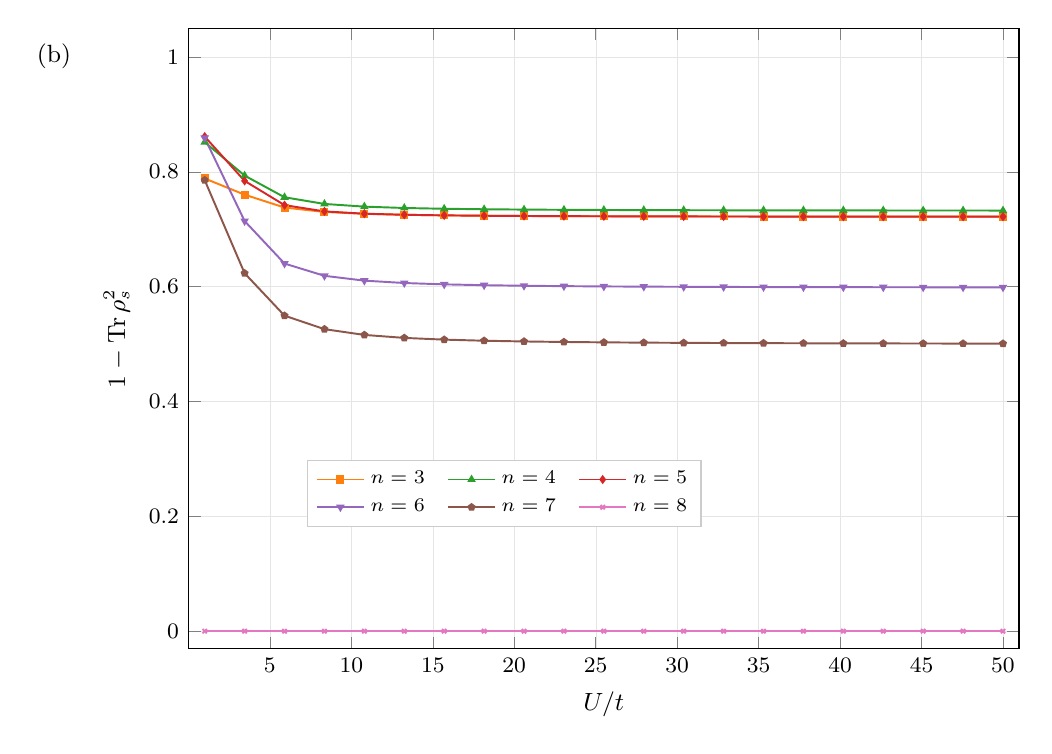
\begin{tikzpicture}
  \begin{axis}[
    width=\columnwidth,
    height=0.78\columnwidth,
    xlabel={$U/t$},
    ylabel={$1-\mathrm{Tr}\,\rho_s^2$},
    grid=both,
    grid style={line width=.1pt, draw=gray!20},
    tick label style={font=\footnotesize\rmfamily, /pgf/number format/fixed},
    label style={font=\small\rmfamily},
    scaled ticks=false,
    legend style={font=\scriptsize\rmfamily, draw=gray!40, at={(0.5,1.03)}, anchor=south, /tikz/every even column/.append style={column sep=6pt}},
    legend cell align={left},
    legend columns=3,
    ymin=-0.03,
    ymax=1.05,
    xmin=0.02,
    xmax=50.98,
    legend style={at={(0.380,0.250)}, anchor=center, fill=white},
    after end axis/.append code={\node[anchor=east, font=\small\rmfamily] at (axis description cs:-0.13,0.954) {(b)};},
  ]
    \addplot[color=gmeC1, mark=square*, mark size=1.1pt, line width=0.7pt] coordinates {
        (1,0.788338) (3.45,0.760102) (5.9,0.737695) (8.35,0.730058)
        (10.8,0.726787) (13.25,0.725089) (15.7,0.724097) (18.15,0.723469)
        (20.6,0.723046) (23.05,0.722749) (25.5,0.722532) (27.95,0.722369)
        (30.4,0.722244) (32.85,0.722145) (35.3,0.722066) (37.75,0.722001)
        (40.2,0.721948) (42.65,0.721904) (45.1,0.721867) (47.55,0.721835)
        (50,0.721808)
    };
    \addlegendentry{$n=3$}
    \addplot[color=gmeC2, mark=triangle*, mark size=1.1pt, line width=0.7pt] coordinates {
        (1,0.85165) (3.45,0.793361) (5.9,0.755606) (8.35,0.744006)
        (10.8,0.73931) (13.25,0.736941) (15.7,0.73558) (18.15,0.734727)
        (20.6,0.734157) (23.05,0.733757) (25.5,0.733467) (27.95,0.733249)
        (30.4,0.733081) (32.85,0.73295) (35.3,0.732844) (37.75,0.732759)
        (40.2,0.732688) (42.65,0.73263) (45.1,0.73258) (47.55,0.732539)
        (50,0.732503)
    };
    \addlegendentry{$n=4$}
    \addplot[color=gmeC3, mark=diamond*, mark size=1.1pt, line width=0.7pt] coordinates {
        (1,0.861283) (3.45,0.78411) (5.9,0.741915) (8.35,0.731)
        (10.8,0.727016) (13.25,0.725121) (15.7,0.724069) (18.15,0.723423)
        (20.6,0.722998) (23.05,0.722703) (25.5,0.72249) (27.95,0.722332)
        (30.4,0.72221) (32.85,0.722115) (35.3,0.722039) (37.75,0.721977)
        (40.2,0.721927) (42.65,0.721885) (45.1,0.721849) (47.55,0.721819)
        (50,0.721793)
    };
    \addlegendentry{$n=5$}
    \addplot[color=gmeC4, mark=triangle*, mark size=1.1pt, mark options={rotate=180}, line width=0.7pt] coordinates {
        (1,0.858872) (3.45,0.714221) (5.9,0.640175) (8.35,0.618834)
        (10.8,0.610437) (13.25,0.606289) (15.7,0.603939) (18.15,0.60248)
        (20.6,0.601511) (23.05,0.600836) (25.5,0.600347) (27.95,0.59998)
        (30.4,0.599699) (32.85,0.599479) (35.3,0.599303) (37.75,0.59916)
        (40.2,0.599042) (42.65,0.598945) (45.1,0.598862) (47.55,0.598792)
        (50,0.598733)
    };
    \addlegendentry{$n=6$}
    \addplot[color=gmeC5, mark=pentagon*, mark size=1.1pt, line width=0.7pt] coordinates {
        (1,0.785367) (3.45,0.623304) (5.9,0.549442) (8.35,0.525947)
        (10.8,0.515907) (13.25,0.510717) (15.7,0.507697) (18.15,0.50579)
        (20.6,0.504511) (23.05,0.503612) (25.5,0.502957) (27.95,0.502465)
        (30.4,0.502086) (32.85,0.501788) (35.3,0.501549) (37.75,0.501355)
        (40.2,0.501196) (42.65,0.501063) (45.1,0.500951) (47.55,0.500855)
        (50,0.500774)
    };
    \addlegendentry{$n=7$}
    \addplot[color=gmeC6, mark=x, mark size=1.1pt, line width=0.7pt] coordinates {
        (1,0) (3.45,0) (5.9,0) (8.35,0)
        (10.8,0) (13.25,0) (15.7,0) (18.15,0)
        (20.6,0) (23.05,0) (25.5,-0) (27.95,-0)
        (30.4,-0) (32.85,0) (35.3,-0) (37.75,0)
        (40.2,0) (42.65,0) (45.1,0) (47.55,0)
        (50,0)
    };
    \addlegendentry{$n=8$}
  \end{axis}
\end{tikzpicture}
